\documentclass[12pt]{article}
%%%%%%%%%%%%%%%%%%%%%%%%%%%%%%%%%%%%%%%%%%%%%%%%%%%%%
%%%%%%%%%%%  MATH  %%%%%%%%%%%%%%%%%%%%%%%%%%%%%%%%%%
\usepackage{amsmath,amsthm,amssymb} %math
\usepackage{xfrac} %sfrac
\usepackage{faktor} %better than sfrac
\usepackage{dutchcal} %some font for mathcal
\usepackage{array}
%\everymath{\displaystyle} %to show every math big
%%%%%%%%%%%%%%%%%%%%%%%%%%%%%%%%%%%%%%%%%%%%%%%%%%%%%
%%%%%%%%%%%  OTHER PACKAGES  %%%%%%%%%%%%%%%%%%%%%%%%
\usepackage[utf8]{inputenc} %encoding
\usepackage{geometry} %page size and margins
\usepackage{makeidx} %indexing
\usepackage{graphicx} %inclusion of graphics
\usepackage{wrapfig} %wrap text around figures
\usepackage{xstring} %manipulate strings
%%%%%%%%%%%%%%%%%%%%%%%%%%%%%%%%%%%%%%%%%%%%%%%%%%%%%
%%%%%%%%%%%  TIKZ 4 LIFE  %%%%%%%%%%%%%%%%%%%%%%%%%%%
\usepackage{tikz}
\usetikzlibrary{cd} %commutative diagrams
\usetikzlibrary{decorations} %curved lines
\usetikzlibrary{positioning} %coordinates positioning
%\usetikzlibrary{replacements} %right=of nodename
\usetikzlibrary{3d,calc} %coordinate calculations & 3d
%%%%%%%%%%%%%%%%%%%%%%%%%%%%%%%%%%%%%%%%%%%%%%%%%%%%%
%%%%%%%%%%%  CUSTOMIZE THE LOOKS  %%%%%%%%%%%%%%%%%%%
\geometry{headheight=15pt}
\setlength\parindent{0pt} %no indentation
%%%%%%%%%%%%%%%%%%%%%%%%%%%%%%%%%%%%%%%%%%%%%%%%%%%%%
%%%%%%%%%%%  ENUMERATE / ITEMIZE  %%%%%%%%%%%%%%%%%%%
\usepackage{enumerate} %enumerate/itemize (has to be first)
\usepackage{enumitem} %customize enumerate/itemize
 \setlist{nolistsep} %<=> [nosep] <=> Kills vert sep <=> ![listsep]
\newenvironment{n_enum}{\begin{enumerate}[label=(\arabic{*})]}{\end{enumerate}} %1,2,3,...
\newenvironment{i_enum}{\begin{enumerate}[label=(\roman{*})]}{\end{enumerate}} %i,ii,iii,...
\newenvironment{a_enum}{\begin{enumerate}[label=(\alph{*})]}{\end{enumerate}} %a,b,c,...
\newenvironment{b_item}{\begin{itemize}}{\end{itemize}} %bullets
%%%%%%%%%%%%%%%%%%%%%%%%%%%%%%%%%%%%%%%%%%%%%%%%%%%%%
%%%%%%%%%%%  MATH NOTATIONS  %%%%%%%%%%%%%%%%%%%%%%%%
\newenvironment{eqarray}{\begin{array}{>{\displaystyle}r>{\displaystyle}c>{\displaystyle}l}}{\end{array}}
\newcommand\Hom{\mathrm{Hom}}
\newcommand\NHom{\mathrm{NHom}}
\newcommand\ChRmod{Ch($R$-mod)}
\newcommand\ChZmod{Ch($\mathbb{Z}$-mod)}
\newcommand\KRmod{$\mathcal{K}$($R$-mod)}
\newcommand\Csing[1]{C^{\mathrm{sing}}\left(#1\right)}
\newcommand\Dtop[1]{\Delta^{\mathrm{top}}\left(#1\right)}
\newcommand\Tor{\mathrm{Tor}}
\newcommand\Ext{\mathrm{Ext}}
\newcommand\Mod{\mathrm{Mod}}
\newcommand\Ab{\mathrm{Ab}}
\newcommand\map{\mathrm{map }}
\newcommand\im{\mathrm{im\ }}
\newcommand\tensor{\otimes}
%\newcommand\ker{\mathrm{ker}}
\newcommand\coim{\mathrm{coim\ }}
\newcommand\coker{\mathrm{coker\ }}
\newcommand\cupdot{\mathbin{\mathaccent\cdot\cup}}
\newcommand\rank{\mathrm{rank}}
\newcommand\val{\mathrm{val}}
%%%%%%%%%%%%%%%%%%%%%%%%%%%%%%%%%%%%%%%%%%%%%%%%%%%%%
%%%%%%%%%%%  OTHER NOTATIONS  %%%%%%%%%%%%%%%%%%%%%%%
\newcommand\ul[1]{\emph{#1}}
\newcommand\nospace{\hspace*{-0.5em}}
\newcommand\HRule{\rule{\linewidth}{0.1mm}}
%%%%%%%%%%%%%%%%%%%%%%%%%%%%%%%%%%%%%%%%%%%%%%%%%%%%%
%%%%%%%%%%%  BEGIN DOCUMENT  %%%%%%%%%%%%%%%%%%%%%%%%
\begin{document}
\begin{center}
{\bf Mathematical Aspects of Public Transportation Networks}\\
Problem Set 8
\end{center}
So 2018 \hfill Dimitrios Bogiokas - BMS\\
\phantom{X}\hfill FU ID: 5048996\\
\HRule\\
{\bf Exercise 1} \begin{a_enum} \item Let $C$ be a cycle basis of $G$, with cycle matrix $\Gamma$. Then $\Gamma\in\{-1,0,1\}^{C\times E}$. Each entry of $\Gamma\cdot A^T\in\mathbb{Q}^{C\times V}$ equals to $c_i^T\cdot p_j$, where $c_i$ is the oriented edge-incidence vector of the $i$-th cycle in $C$ and $p_j$ is the oriented edge-incidence vector of the $j$-th vertex. Thus, the only edges that affect the inner product $c_i^Tp_j$ are those edges of the cycle $i$, which are incident to the vertex $j$. Since $j$ is a cycle, i.e. an Eulerian subgraph of $G$, these edges come in pairs, every time that the associated Eulerian cycle enters and exits the vertex $j$. If both of them are in-edges or if both of them are out-edges of vertex $j$, then they both have the same value in $p_j$ ($1$ or $-1$ respectively) and their sign differs in $c_i$. If the one is an in-edge and the other an out-edge of vertex $j$, the sign of their respective entries differs in $p_j$, but they have the same value in $c_i$. In either case, the sum of the pairwise product of these entries vanishes, proving that $c_i^Tp_j=0$ and thus:
$$\Gamma\cdot A^T = 0_{C\times V}$$
\item ($\Leftarrow$) Let $G'=G[e_1,\ldots,e_k]$ be the directed subgraph induced by this edge set. Then the incident matrix $A'$ of $G'$ has the collumns $a_1,\ldots,a_k$ (up to a permutation). Let $C'$ be a cycle basis of $G'$ and
$$\Gamma'=\left(\begin{array}{c}c_1\\\hline\vdots\\\hline c_{\mu'}\\\end{array}\right)\in\{-1,0,1\}^{[\mu']\times[k]}$$
be the respective cycle matrix, where $\mu'=|C'|$ and the above is a block notation of $\Gamma'$. Let $c$ be a cycle in $G'$. This means that there exists a vector $(\lambda_1,\ldots,\lambda_{\mu'})\in\mathbb{Q}^{1\times\mu'}$, such that:
$$c=(\lambda_1,\ldots,\lambda_{\mu'})\cdot\Gamma'\in\mathbb{Q}^k$$
This means that
$$c\cdot\left(\begin{array}{c}a_1\\\hline\vdots\\\hline a_k\\\end{array}\right)=(\lambda_1,\ldots,\lambda_{\mu'})\cdot\Gamma'\cdot A'^T\overset{\text{(a)}}{=}0_{1\times V(G')}$$
which is a vanishing non-zero linear combination of $a_1,\ldots a_k$, making this set $\mathbb{Q}$-linear dependent.\\
($\Rightarrow$) Let $e_1,\ldots,e_k\in E$ be such that $G'=G[e_1,\ldots,e_k]$ contains no cycles and let $\lambda_1,\ldots,\lambda_k\in\mathbb{Q}$, s.t.
$$(\lambda_1,\ldots,\lambda_k)\cdot A'^T=(\lambda_1,\ldots,\lambda_k)\cdot\left(\begin{array}{c}a_1\\\hline\vdots\\\hline a_k\end{array}\right)=\lambda_1a_1+\lambda_2a_2+\cdots+\lambda_ka_k=0_{1\times V(G')}$$
We will show that $\lambda_1=\cdots=\lambda_k=0$. Since $G'$ contains no cycle, it is a forest and thus it has at least one leaf, i.e. a vertex $v\in V(G')$ of degree $1$. Let $e_i$ be the adjacent edge to $v$. Then, the $v$-th entry of $(\lambda_1,\ldots,\lambda_k)\cdot A'^T$ equals $\lambda_i$ (since $e_i$ is the only adjacent edge of $v$). This means that $\lambda_i=0$. Removing the vertex $v$ from $G'$, we get another cycle-free graph $G''=G'\setminus v$, which contains every other edge, except for $\lambda_i$. Let $A''$ be $A'$ without the collumn $a_i$. Then the equation $(\lambda_1,\ldots,\hat{\lambda}_i,\ldots,\lambda_k)\cdot A''^T=0$ still holds in $G''$. After $V(G')-1$ iterations there will be no edge left in the graph and thus everyone among $\lambda_1,\ldots,\lambda_k$ is proven eventually to be zero. This proves that there does not exist a $\mathbb{Q}$-linear dependance of $a_1,\ldots,a_k$, finishing the proof.
\item Let $G$ be a directed graph with incident matrix $A$, and let $\Gamma$ be a cycle matrix of some cycle basis of $G$. Let $a_1,\ldots,a_n\in\mathbb{Q}^{E}$ be the rows of $A$ and $c_1,\ldots,c_{m-n+c}\in\mathbb{Q}^E$ the rows of $\Gamma$, where $n,m$ and $c$ are the number of vertices, edges and weakly connected components of $G$, respectively (we do not need that $c=1$). Then, almost by definition we have:
$$\rank\Gamma=\dim_{\mathbb{Q}}\mathcal{C}_{\mathbb{Q}}(G)=\mu(G)=m-n+c$$
and from (b) we have:
$$\rank A=\max\{k:\text{ there exist }k\ \mathbb{Q}\text{-lin. ind. rows of }A\}=n-c$$
because every maximal set of edges in $G$, which do not include a cycle forms a spanning forest, which has $n-c$ edges. Moreover, from (a) we get:
$$a_i^T\cdot c_j=0\ \forall(i,j)\in[m-n+c]\times[n-c]$$
Thus, the rows of $\Gamma$ and $A$ span two perpendicular subspaces of $\mathbb{Q}^m$ of dimensions $m-n+c$ and $n-c$ respectively, which proves that:
$$\left<a_1,\ldots,a_{n-c},c_1,\ldots,c_{m-n+c}\right>\cong\mathbb{Q}^{n-c+m-n+c}=\mathbb{Q}^m$$
\end{a_enum}
\ \\
{\bf Exercise 2} Let $A\in\mathbb{Q}^{m\times n}$ and $b\in\mathbb{R}^m$.
\begin{a_enum} 
\item Let moreover $x\in Q(A,b)$. We will show that $x\in P(A,b)$: Let us first define for each $i\in[m]$ the positive integer $r_i$ as the least common factor of all denominators of every entry in row $i$ of $A=(a_{ij})_{i\in[m],j\in[n]}$:
$$r_i:=\min\{t\in\mathbb{Z}_+:ta_{ij}\in\mathbb{Z}\ \forall j\in[n]\}$$
Fix now some $s\in[m]$ and define the vector $\lambda^{(s)}=\left(\lambda^{(s)}_i\right)_{i\in[m]}$, with $\lambda^{(s)}_i:=r_se_i$, i.e. $\lambda^{(s)}$ has every coordinate equal to zero, except for the $s$-th one, which is equal to $r_s$. For our choice $x$, we know in particular that:
$$\left(\lambda^{(s)}\right)^TAx\leq\left\lfloor\left(\lambda^{(s)}\right)^Tb\right\rfloor\ \ \forall s\in[m]$$
Define the integer matrix $A':=(r_ia_{ij})_{i\in[m],j\in[n]}$ and the vector $b'=(r_ib_i)_{i\in[m]}\in\mathbb{R}^m$. Notice that $P(A,b)=P(A',b')$, since we just multiplied each inequality with some positive number. Notice now that the above $m$ inequalities for x can be summarized to:
$$A'x\leq\lfloor b'\rfloor\leq b'$$
which means that $x\in P(A',b')=P(A,b)$, proving the assertion.
\item Let now $x\in P(A,b)\cap\mathbb{Z}^n$. This means that $Ax\leq b$, and thus we also have $\lambda^TAx\leq\lambda^Tb$, for every $\lambda\geq0$. If $\lambda^TA$ has integer entries, since $x$ is also an integer vector, the LHS is an integer, for every inequality $1,\ldots,m$. Thus, $\lambda^TAx\leq\lfloor \lambda^Tb\rfloor$, i.e. $x\in Q(A,b)$.
\item Let $\lambda=(\gamma_+^T,\gamma_-^T)^T\in\{0,1\}^{2m}$. Obviously $\lambda\geq0$ and $\lambda^TA\in\mathbb{Z}^{n+m}$, since $A$ has also integer entries. This means, that for every $(\pi,p)\in Q(A,b)$ we get (in block-matrix notation):
$$\begin{array}{c>{\displaystyle}rc>{\displaystyle}l}&\lambda^TA\left(\begin{array}{c}\pi\\p\\\end{array}\right)&\leq&\lfloor\lambda^Tb\rfloor\\
\Rightarrow&(\gamma_+^T,\gamma_-^T)\left(\begin{array}{c|c}B&T\cdot I_m\\\hline-B&-T\cdot I_m\\\end{array}\right)\left(\begin{array}{c}\pi\\p\\\end{array}\right)&\leq&\left\lfloor(\gamma_+^T,\gamma_-^T)\left(\begin{array}{c}u\\-l\\\end{array}\right)\right\rfloor\\
\Rightarrow&\left(\begin{array}{c|c}\gamma_+^TB-\gamma_-^TB&T\cdot\gamma_+^TI_m-T\cdot\gamma_-^TI_m\\\end{array}\right)\left(\begin{array}{c}\pi\\p\\\end{array}\right)&\leq&\left\lfloor\gamma_+^Tu-\gamma_-^Tl\right\rfloor\\
\Rightarrow&\left(\begin{array}{c|c}\gamma^TB&T\cdot\gamma^TI_m\\\end{array}\right)\left(\begin{array}{c}\pi\\p\\\end{array}\right)&\leq&\left\lfloor\gamma_+^Tu-\gamma_-^Tl\right\rfloor\\
\overset{(1)}{\Rightarrow}&T\cdot\gamma^Tp&\leq&\left\lfloor\gamma_+^Tu-\gamma_-^Tl\right\rfloor\\
\overset{(2)}{\Rightarrow}&\gamma^Tp&\leq&\left\lfloor\frac{\gamma_+^Tu-\gamma_-^Tl}{T}\right\rfloor\\
\end{array}$$
Where, $(1)$ is true because $\gamma^TB=0\in\mathbb{R}^n$, like we showed in the first exercise and $(2)$ is true because $\gamma^Tp\in\mathbb{Z}$: Let $n\in\mathbb{Z}$, $a,x\in\mathbb{R}$. Then $n\leq a\lfloor x\rfloor$ gives $n\leq\lfloor ax\rfloor$. Indeed:
$$n\leq a\lfloor x\rfloor\overset{n\in\mathbb{Z}}{\Rightarrow}n\leq\lfloor a\lfloor x\rfloor\rfloor\overset{\lfloor x\rfloor\leq x}{\leq}n\leq\lfloor ax\rfloor$$
\end{a_enum}
\ \\
{\bf Exercise 3} \begin{a_enum}
\item Let $s$ be the symmetry axis. Then, we have the following EAN:
\begin{center}
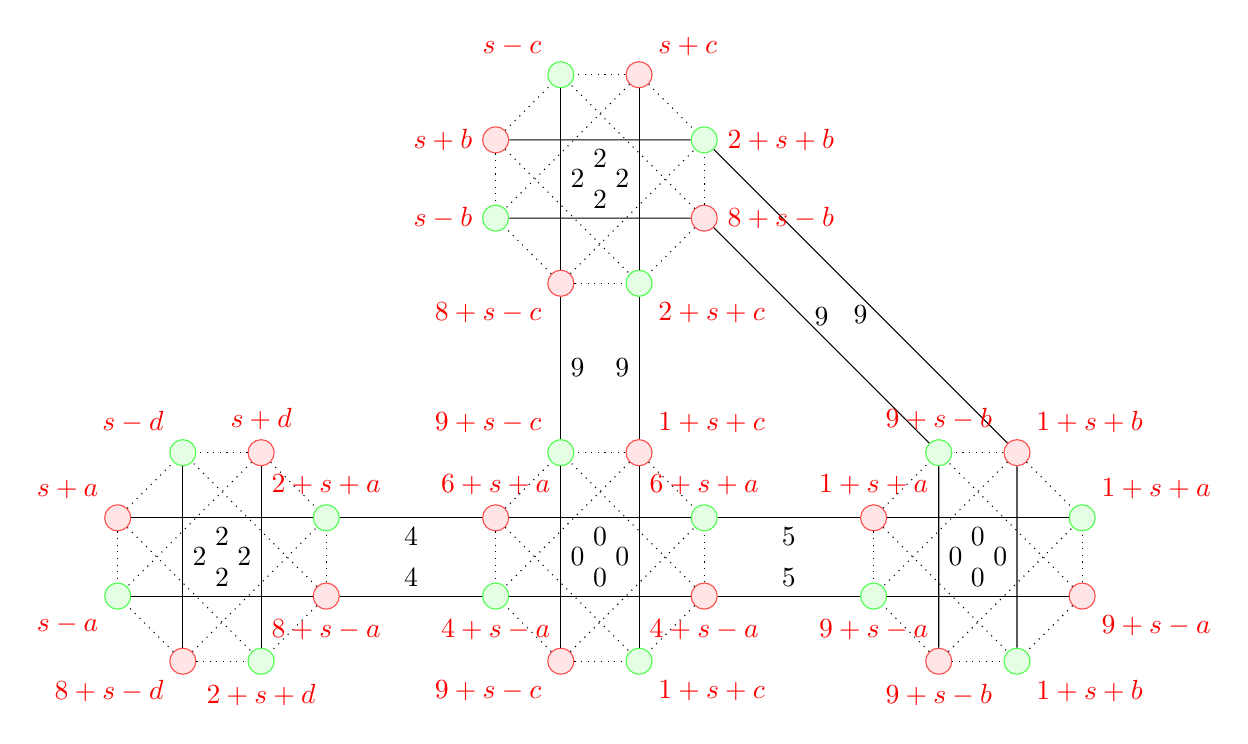
\begin{tikzpicture}[
event/.style={circle,draw,node distance = .2cm},
eventd/.style={draw=green!70,fill=green!10,event},
eventa/.style={draw=red!70,fill=red!10,event},
label/.style={red, node distance = 0cm},
node distance = 1.2cm]
\def\dist{4.8}
\def\a{above}
\def\b{below}
\def\l{left}
\def\r{right}
\def\al{above left}
\def\bl{below left}
\def\ar{above right}
\def\br{below right}
\coordinate (A) at (-\dist,0);
\coordinate (B) at (0,0);
\coordinate (C) at (\dist,0);
\coordinate (D) at (0,\dist);

\foreach\p in {A,B,C,D} {
%	\node at (\p) {\p};
	\node[right=of \p] (\p r)  {};
	\node[eventd] (\p rd) [above=of \p r] {};
	\node[eventa] (\p ra) [below=of \p r] {};
	\node[below=of \p] (\p b)  {};
	\node[eventa] (\p ba) [left=of \p b] {};
	\node[eventd] (\p bd) [right=of \p b] {};
	\node[left=of \p] (\p l)  {};
	\node[eventa] (\p la) [above=of \p l] {};
	\node[eventd] (\p ld) [below=of \p l] {};
	\node[above=of \p] (\p a)  {};
	\node[eventd] (\p ad) [left=of \p a] {};
	\node[eventa] (\p aa) [right=of \p a] {};
	\draw[dotted] (\p ra)--(\p rd);
	\draw[dotted] (\p ra)--(\p bd);
	\draw[dotted] (\p ra)--(\p ad);
	\draw[dotted] (\p ba)--(\p rd);
	\draw[dotted] (\p ba)--(\p bd);
	\draw[dotted] (\p ba)--(\p ld);
	\draw[dotted] (\p la)--(\p bd);
	\draw[dotted] (\p la)--(\p ld);
	\draw[dotted] (\p la)--(\p ad);
	\draw[dotted] (\p aa)--(\p rd);
	\draw[dotted] (\p aa)--(\p ld);
	\draw[dotted] (\p aa)--(\p ad);
}
\draw (Ala)--node[below] {2} (Ard)--node[below] {4} (Bla)--node[below] {0} (Brd)--node[below] {5} (Cla)--node[below] {0} (Crd);
\draw (Cra)--node[above] {0} (Cld)--node[above] {5} (Bra)--node[above] {0} (Bld)--node[above] {4} (Ara)--node[above] {2} (Ald);
\draw (Aba)--node[right] {2} (Aad);
\draw (Aaa)--node[left] {2} (Abd);
\draw (Bba)--node[right] {0} (Bad)--node[right] {9} (Dba)--node[right] {2} (Dad);
\draw (Daa)--node[left] {2} (Dbd)--node[left] {9} (Baa)--node[left] {0} (Bbd);
\draw (Cba)--node[right] {0} (Cad)--node[above] {9} (Dra)--node[above] {2} (Dld);
\draw (Dla)--node[below] {2} (Drd)--node[below] {9} (Caa)--node[left] {0} (Cbd);
\node[label] [\al=of Ala] {$s+a$};
\node[label] [\bl=of Ald] {$s-a$};
\node[label] [\a=of Ard] {$2+s+a$};
\node[label] [\b=of Ara] {$8+s-a$};
\node[label] [\a=of Bla] {$6+s+a$};
\node[label] [\b=of Bld] {$4+s-a$};
\node[label] [\a=of Brd] {$6+s+a$};
\node[label] [\b=of Bra] {$4+s-a$};
\node[label] [\a=of Cla] {$1+s+a$};
\node[label] [\b=of Cld] {$9+s-a$};
\node[label] [\ar=of Crd] {$1+s+a$};
\node[label] [\br=of Cra] {$9+s-a$};
\node[label] [\l=of Dla] {$s+b$};
\node[label] [\l=of Dld] {$s-b$};
\node[label] [\r=of Drd] {$2+s+b$};
\node[label] [\r=of Dra] {$8+s-b$};
\node[label] [\ar=of Caa] {$1+s+b$};
\node[label] [\a=of Cad] {$9+s-b$};
\node[label] [\br=of Cbd] {$1+s+b$};
\node[label] [\b=of Cba] {$9+s-b$};
\node[label] [\ar=of Daa] {$s+c$};
\node[label] [\al=of Dad] {$s-c$};
\node[label] [\br=of Dbd] {$2+s+c$};
\node[label] [\bl=of Dba] {$8+s-c$};
\node[label] [\ar=of Baa] {$1+s+c$};
\node[label] [\al=of Bad] {$9+s-c$};
\node[label] [\br=of Bbd] {$1+s+c$};
\node[label] [\bl=of Bba] {$9+s-c$};
\node[label] [\a=of Aaa] {$s+d$};
\node[label] [\al=of Aad] {$s-d$};
\node[label] [\b=of Abd] {$2+s+d$};
\node[label] [\bl=of Aba] {$8+s-d$};
\end{tikzpicture}
\end{center}
where the arrival events are red and the departure events are green. The red labels are the values of any timetable, depending on $s$ and four parameters $a,b,c,d$, one for each line. The slack depends only on $a,b,c,d$, since each action has a value of the form $s+$sth. The minimum weighted periodic slack is $132$ and the proof has the form of a C++ program, also sent to you. 
\end{a_enum}
\end{document}
